% !TEX root = ./summary.tex

\section{Abstrakter Syntax Baum visualisieren}
\label{sec:visualizeAST}
Hier geht es darum den zu zeigen, wie man den Abstrakten Syntax Baum mithilfe von \antlr zu visualisieren. Im Folgenden wird der Abstrakter Syntax Baum als AST f"ur abstract syntax tree genutzt. 

\subsection{Vorgehen}
Den AST mithilfe von \antlr zu visualisieren ist ziemlich einfach. Man benutzt eine Hilfsklasse, die das f"ur einen "ubernimmt. 

\begin{lstlisting}[language=Java]
public class VisualAST_Main {
    public static void main(String[] args) {
	args = new String[4];
	args[0] = "ch.hsr.compB.parser.Demo";
	args[1] = "addition";
	args[2] = "-gui";
	args[3] = "target/code.demo";
	    try {
		org.antlr.v4.gui.TestRig testRig = 
		    new org.antlr.v4.gui.TestRig(args); 
		testRig.process();
	    } catch (Exception e) {
		e.printStackTrace();
	    }
    }
}
\end{lstlisting}

\paragraph{Bemerkung:}
Hier merkt man dann, wenn man die falsche bzw. alte \antlr Library eingebunden hat. Die Klasse TestRig l"asst sich n"amlich nicht finden in dem Package org.antlr.v4.gui. Es wird eine Meldung angegeben, dass diese Klasse nicht gefunden wird. Sobald man aber die richtige Library bei dem Plugin angegeben hat, sollte es funktionieren

Die Argumente, die die Klasse TestRig braucht sind zum einen das von \antlr generierte Tokenfile, sowie sie erste Regel der Grammatik aus dem .g4 File. Das -gui bedeutet, dass der Baum visualisiert werden soll und das letzte Argument, ist ein Input der im File .demo daher kommt.

Der AST k"onnte ungef"ahr so aussehen:

\begin{figure}[H]
	\centering
	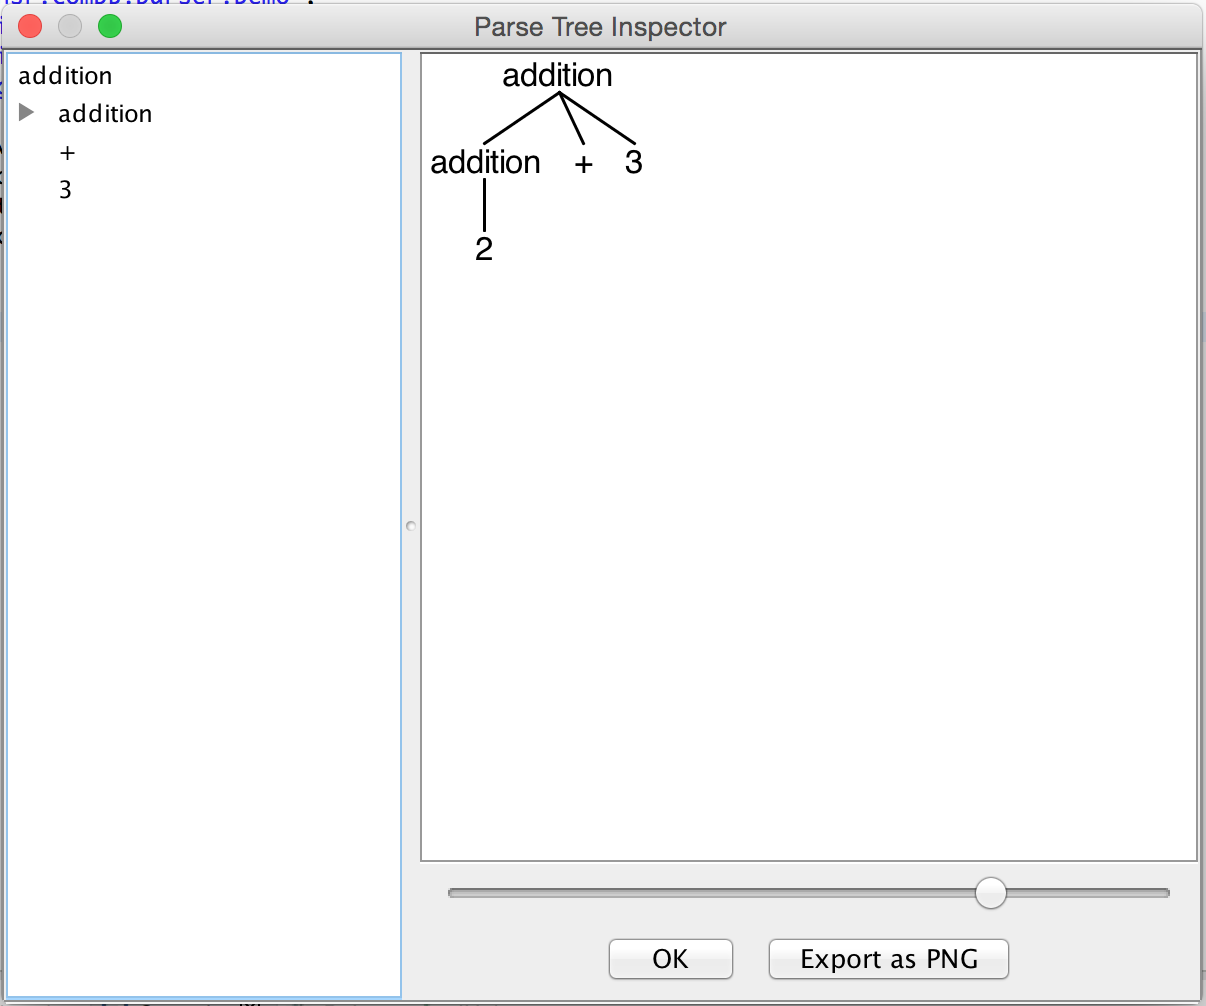
\includegraphics[width=0.65\textwidth]{my_ast}
	\caption{Der AST von 2+3}
\end{figure}

Wenn man es genau nimmt, dann ist das eigentlich gar kein AST sondern ein Parsetree. Der unterschied besteht im wesentlichen, dass bei einem AST das Plus ein Knoten darstellen w"urde, und die Zahlen die Bl"atter

\begin{figure}[H]
	\centering
	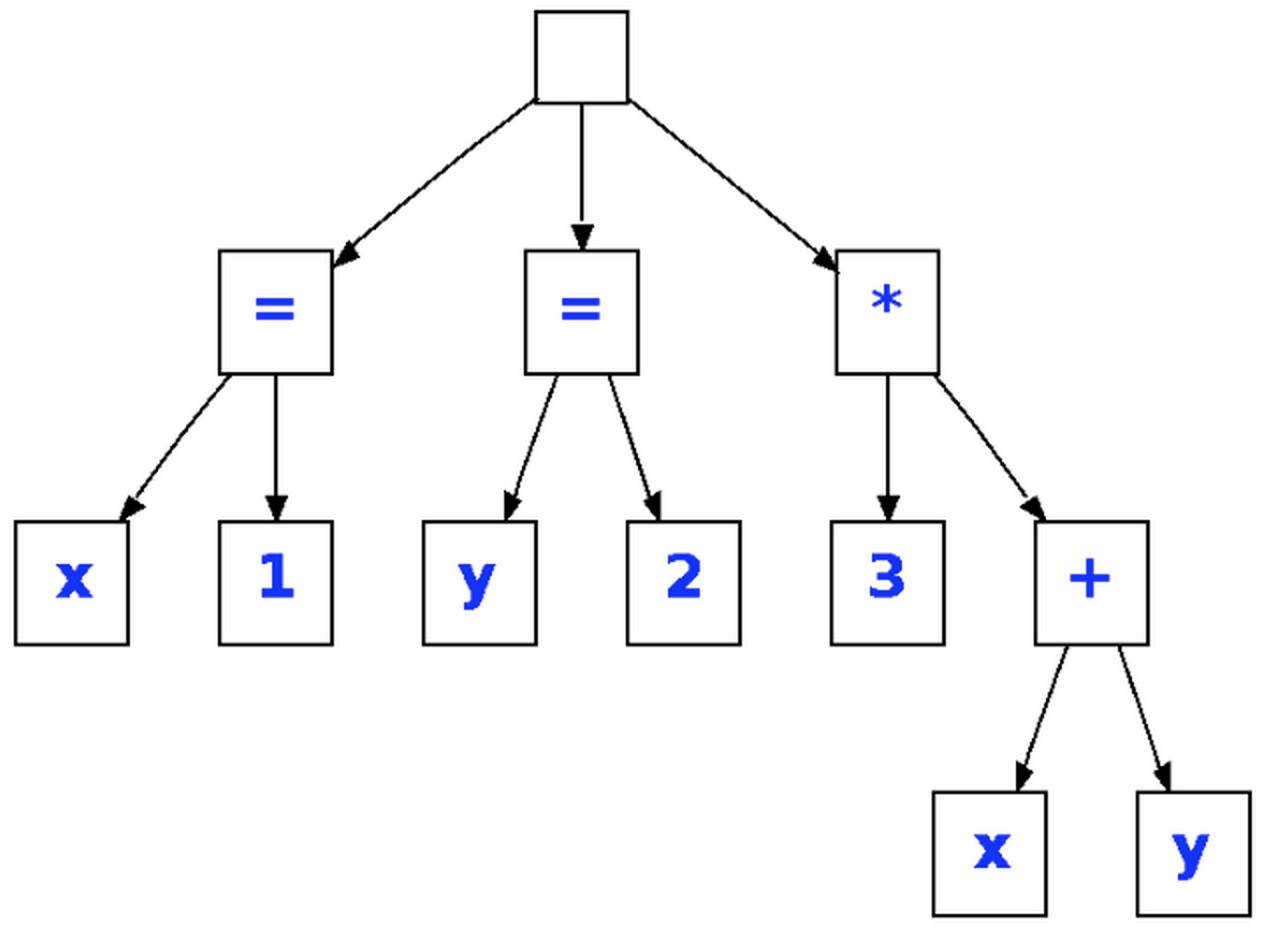
\includegraphics[width=0.65\textwidth]{ast_stacko}
	\caption{Einen richtigen AST des Inputs x=1, y=2, 3*(x+y)}
\end{figure}

Das Bild stammt von hier\footnote{Quelle:\\ \url{http://stackoverflow.com/questions/5026517/whats-the-difference-between-parse-tree-and-ast}} und wer mehr dar"uber wissen will, kann dort noch mehr dazu lesen.











